\subsection{Development Process}
Since we are not developing safety critical software, we can use a more agile approach
to developing software, which ensures that we are meeting stakeholder requirements and prioritizing
the most important features. This also allows us to present more concrete software for feedback.
%refacrtor 
%Development process (encompasses too many things), 
%Software developement process?
%Project management 
%Title for tools, prog language, liabaires etc 
%Testing-> can have subsections depending on word count
%Development process -> encompasses meetings, background of members, planned roles as well as linking steps to achieve project goals ?
%Have about 2-3 pages

%can use images for polling to be put in appendix 
\par
The structure to development:\\
\begin{enumerate}
\item Design a suitable interface focusing on the main features to prepare code for use case
\item Create test case for main interface
\item Initial code implementation with test cases for all components added
\item Review code and ensure test cases meet requirements and have high code coverage
\item Add / modify documentation within code to ensure information is accurate
\item Review development process and identify difficulties and effectiveness encountered % ? exapnd on this
\end{enumerate}
\par
For our development process we will be using snake case when writing code as everyone
preferred using it, although a possible alternative is using different casing for
variables and functions should we find using only snake case confusing.
\begin{figure}[h!]
    \centering
    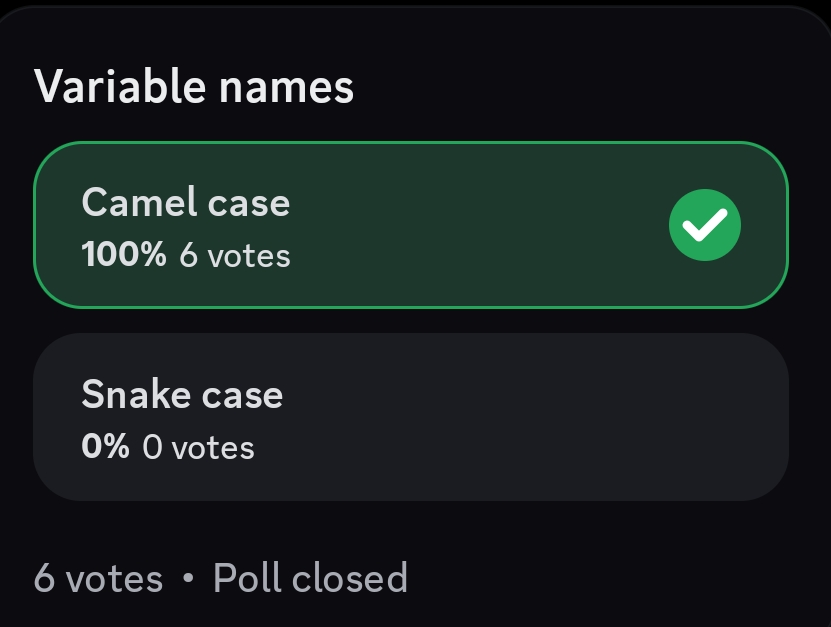
\includegraphics[width=0.5\linewidth]{variableNamingPoll}
    \caption{Poll showing developers opinion on variable naming schemes}
    \label{fig:variableNamingPoll}
\end{figure}
\subsubsection{Team}
For team management, it will be assigned on a per task basis.
This means that the project manager will determine the number of people
and the neccessary roles required for the task.
Members are not restricted to any particular role through the entire project but rather
decide for each task what they will do.
\begin{center}
    \begin{tabular}{|c|c|}
         \hline
         Role & Responsibility \\
         \hline
         Project Manager & Responsible for adapting methods, maintaining contact with\\
         & customer, meeting up with members and creating tasks to complete \\
         \hline
         Programmer & Responsible for writing software and adding documentation as needed\\
         \hline
         Tester & Write test for code, refactor code as deemed necessary and ensure code meets\\
         & agreed standards\\
         \hline
         CI/CD & Responsible for measuring and improving compile times. Adds features to pipeline\\
         & to improve development experience and code quality\\
         \hline
         Designer & Responsible for creating interface and creating diagrams for general structure.\\
         & This could involve UML diagrams or database diagrams etc.\\
         \hline
         
    \end{tabular}
\end{center}

\subsection{Tools}
We will be using Github to track our changes, allowing us to work simultaneously, 
track issues, and keep track of who is working on what. 
Github's CI/CD will also be used to detect any errors added from committed code.
%Split up tasks e.g gantt chart for outline while kanban/trello for development
\par
For scheduling we could use a kanban board to track what tasks need completing and seeing
progress for current tasks. Alternatively we could use Github's issue section to manage
the activities needing completion. This comes at the drawback of being harder to track progress
for.
\par
Using more tools brings more friction to the development process, so to find out our team's
preference a quick poll was asked where everyone agreed % Reference here
\begin{figure}[h!]
    \centering
    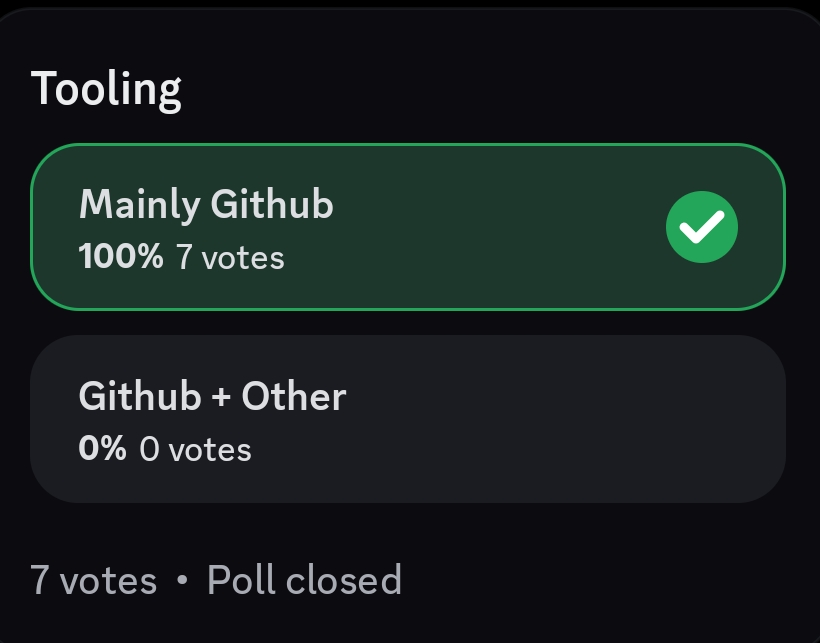
\includegraphics[width=0.5\linewidth]{toolingPoll}
    \caption{Poll showing developers opinion on using tooling}
    \label{fig:toolingPoll}
\end{figure}
to use mainly Github as to have all the information in one centralized tool

%talk about software with mention before 
\par
We will be using Discord to manage communication as it allows for easy organization and
for online meetings should people be unable to attend in person. It allows for polls to
quickly get opinions on decisions being made.
\subsection{Language / Libraries}
For developing Android applications, we can choose from Python using Kivy or Java using the Android SDK.
Python's Kivy module looks to have good documentation\footnote{https://kivy.org/doc/stable/api-kivy.html}.
For Java, there are two possible choices for documentation:
\begin{enumerate}
  \item Using the official Android site
    \footnote{https://developer.android.com/reference/android/package-summary} % Edit to follow ACM
  \item Devdoc provides a simpler alternative
    \footnote{https://devdoc.net/android/Android-r15/reference/android/package-summary.html} % Edit to follow ACM
\end{enumerate}
\par
In order to determine the best language to use, we carried out a poll among the development team,
finding that 67\% of the team wanted to use Java and only one person against it.
\begin{figure}[h!]
    \centering
    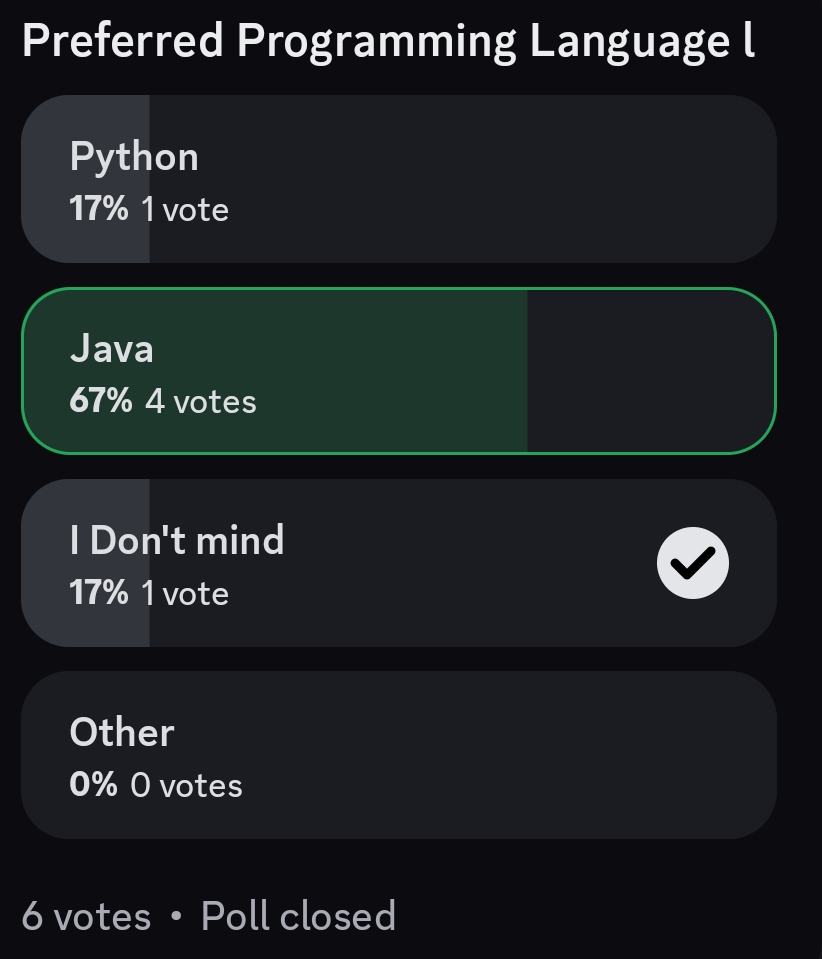
\includegraphics[width=0.5\linewidth]{programmingLanguagePoll}
    \caption{Poll showing developers opinion on programming languages}
    \label{fig:programmingLanguagePoll}
\end{figure}
\par
\subsubsection{Programming Tools}
We will also be using gradlew lint, as the default for Android studio to lint our code
ensuring consistent formatting standard among developers. This is useful as it provides
feedback prior to uploading code. This means that submitted code is less likely to contain
errors
\subsubsection{Libraries}
For libraries used, we will prioritize using popular well-known libraries, as they will have more
active security development reducing the likelihood of vulnerabilities. We will focus on using
open-source libraries which gives us the freedom to modify source code to adjust functionality to
better suit our needs, and to reduce cost, ensuring our product is available for our stakeholders.

\subsection{Testing}
We will be using Github's CI/CD tool to perform automatic regression testing for our software.
This ensures any added code doesn't break previous expectations.
Furthermore, for local development, we will integrate LSPs and formatting tools to quickly detect
simple bugs, as well as to ensure that the code has a consistent style to make navigating and understanding easier.
Beyond that, we will also ensure new features have appropriate tests added, as well as ensuring commits are
reviewed by at least one other person before merging feature to main.

\par
\subsection{Evaluation}
We will focus on customer feedback as well as our test cases to ensure consistent improvement in our software.
% also acceptence
% such as?
For evaluating our work we will be using a testing library such as JUnit. This allows us to:\\
\begin{enumerate}
%refactor
\item Ensure code coverage to ensure all code paths are handled appropriately
\item Provides quick feedback and find regressions added from code
\item Allows us to explicitly verify we are meeting customer requirements, by creating tests specifically for them
\end{enumerate}

\par
Our evaluation process will consist of three main parts:

\begin{enumerate}
\item Efficiency, which is used to identify technical debt build up and enable us to refactor early.
\item Test, to ensure program works as expected
\item Customer reviews, to be able to adapt to possible miscommunications and requirement changes
\end{enumerate}


\subsection{Work Distribution}
%story points fpr deveklopment? Can I discuss about it or is it too early 
To ensure fair distribution of work, we will assign an estimated difficulty level to each task to ensure that
everyone is contributing equally. Due to using agile, we will have short meetings daily, which can be used to
modify the difficulty of a task should it be deemed necessary.
%modify difficulty?
\par
We will avoid assigning specific teams dedicated to certain areas of the project as that could lead to some‪‬

people waiting on others to be able to work, and could lead to burn out. By giving people unrestricted access
to any task, it ensures multiple people are looking over the code, preventing technical debt as well as ensuring
everyone is familiar with the code base, so should someone fall ill, there will be minimal productivity disruption.
%Yes but need to refactor, can allude to sub specific, documentation?

